\section{Inhomogeneous Linear Systems}
Suppose we have an equation of the form
\begin{equation}\label{eq:inhom-ode}
    X' = Ax + f(t)
\end{equation}
Then we know from the superposition principle (see \autoref{sec:superposition-principle}) that the general solution to this system is given by
$$ X(t) = y(t) + e^{tA}v $$
where $y(t)$ is a particular solution to the ODE and $v$ is some arbitrary vector that is determined by the initial conditions. Thus our goal is to find just \textit{one} solution to this ODE. This leads us to Duhamel's Principle.

\subsection{Duhamel's Principle}
We will guess that $y(t) = e^{tA} v(t)$ is a solution where $v(t)$ is a function to be determined (this is the technique of variation of constants). Assuming $y$ is a solution we can plug this in \autoref{eq:inhom-ode} to find the left and right hand sides are
\begin{align}
    y' &= Ae^{tA} v(t) + e^{tA} v'(t) \tag{LHS}\\
    Ay + f(t) &= Ae^{tA} v(t) + f(t) \tag{RHS}
\end{align}
Equating the two we find that
$$ v'(t) = e^{-tA} f(t) $$
Hence by the Fundamental Theorem of Calculus we find that 
$$ v(t) = \int_{0}^{t} e^{-sA} f(s) ds $$
(recall we only need a particular solution so we can ignore the constant of integration by setting it to 0). 
Therefore our particular solution $y$ is given by
$$ y(t) = e^{tA} v(t) = e^{tA} \int_{0}^t e^{-sA} f(s) ds = \int_{0}^t e^{(t - s)A} f(s) ds $$
\begin{remark}
Note that $t - s$ is always positive. Although not particularly relevant to this example, this is an important note in other contexts.
\end{remark}
\begin{remark}
What we mean by integrating a vector-valued function is to integrate each of the component functions and `stack' them together to get another vector.
\end{remark}

\section{Linearisation}
The idea with linearisation is to try and use the framework we've built up thus far to make statements about non-linear systems.
Suppose $f: \R^n \to \R^n$ is a smooth vector field and we have the differential equation
\begin{equation}\label{eq:linsation-eg}
    x' = f(x)
\end{equation}
Although in general it's hard to give an explicit solution to this, we can still try and determine it's qualitative behaviour, at least locally. Let $p \in \R^n$ be arbitrary. If $f(p)$ is non-zero, then for $q$ near $p$ we are going to have that $f(q)$ is close to $f(p)$. Therefore the flow is going to look like (almost) parallel lines in this neighbourhood. If $f(p)$ is 0, we need to do a bit more work. One thing we can do is consider the Taylor expansion of $f$. We know that
$$ f(x) = f(p) + f'(p)(x - p) + \underbrace{O(\left|x - p\right|)}_{\text{error}} $$
Since we assume $f(p) = 0$, the first term disappears and by substituting $y = x - p$, \autoref{eq:linsation-eg} becomes
$$ y' = Df(p)y + O(\left|y\right|) $$
Since $Df(p)$ is a linear map, this looks just like the linear equations we have studied thus far, except there is the added error term. The hope is that this error terms is going to be small so by studying the linear system
$$ y' = Df(p) y $$
we can get a pretty good idea of how the true system behaves. For example if there are sources or sinks in the linearised system, they will also appear in the true system. The phase portraits will also be similar (similarity will be defined more precisely later) if the origin is hyperbolic (recall this means that $\Re(\lambda) \neq 0$ for every eigenvalue $\lambda$ of $Df(p)$).

This determines a procedure that we can use to study such equations
\begin{minenumerate}
    \item Find the steady states/equlibria (the points where $x' = f(x)$ is 0). These are points where the solutions are constant and don't change over time.
    \item Linearise near these steady states
    \item Tie everything up into a big picture
\end{minenumerate}
The cryptic `tie everything up into a big picture' can be best illustrated with an example.

\subsection{Example}
We will consider the case of swinging a pendulum, kind of. More precisely we will look at the case when a mass is attached to a (rigid) rod allowed to swing freely in a vertical circle (we use a rod instead of a string because we don't want to worry about cases where the string may fold onto itself or something). 

\begin{figure}[ht]
    \centering
    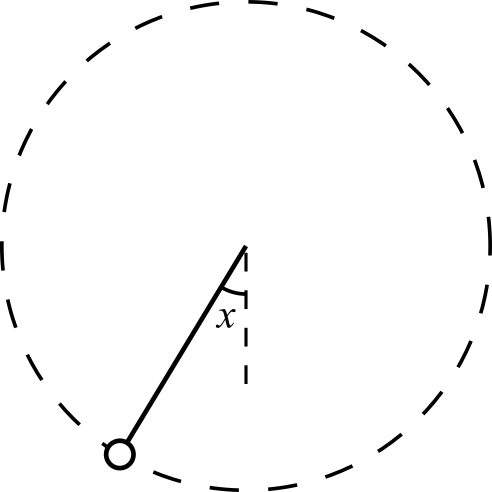
\includegraphics[scale=0.7]{Images/mass_pendulum_diagram.png}
    \caption{Mass pendulum setup}
    \label{fig:mass-pend-diagram}
\end{figure}

The equation modelling this situation is given by
\begin{equation*}
    mx'' + rx' = -c \sin x
\end{equation*}
where $x$ is the angle made by the rod with the vertical. Here $m$ is the mass of the mass (names are difficult for physicists), $r$ is the constant of friction (therefore $r \geq 0$) and $c$ is some arbitrary constant (the exact details, such as length of the rod, strength of gravity, etc, are used to set $c$). To make the analysis a bit simpler we will assume $m$ and $c$ to be 1. Then in particular we have the equation
\begin{equation}
    x'' + rx' + \sin x = 0
\end{equation}
We can use our standard trick to convert this second order equation to a system of first order equation: let $v = x'$. Then we have
\begin{align*}
    \begin{cases}
    x' &= v\\
    v' &= -rv - \sin x
    \end{cases}
\end{align*}
We first find the the steady states or in other words where $v$ is 0 (this implies that $v'$ is 0 since $v' = \frac{df(x(t))}{dt} = f'(x) x'(t) = f'(x) v = 0$. These are the points where $\sin x = 0$ or in other words where $x = k\pi, k \in \Z$. $k$ being even corresponds with the mass hanging on the bottom and $k$ being odd is when the mass is at the top in a perfectly vertical position. Simple intuition tells us that the the former equlibria should be stable (at least if $r > 0$)and the latter should be unstable. Let us see if the equations agree with this. First we see that 
$$ \matrix{x\\v}' = f(x,v), f(x, v) = \matrix{v\\-rv - \sin x}$$
Then
\begin{align*}
    Df(k\pi, 0) &= \matrix{0 & 1\\-\cos x & -r}\Bigg|_{x = k\pi}\\
    &= 
    \begin{cases}
    \matrix{0 & 1\\1 & -r}, &k \text{ odd}\\
    \matrix{0 & 1\\-1 & -r}, &k \text{ even}
    \end{cases}
\end{align*}

Let us consider the case with $k$ odd first. In this case the determinant of the matrix is $-1$ so the eigenvalues are real and of opposite sign. We know this will result in a saddle and hence be unstable. In fact around these points we expect the phase portrait to (roughly) have a saddle as well. This lines up with our intuition above.

Now let us consider the case with $k$ even. Then we know the eigenvalues are
$$ \lambda_{1, 2} = \frac{-r \pm \sqrt{r^2 - 4}}{2} $$
If $0 < r < 2$ then we will have complex eigenvalues implying that we will have a spiral. Since the real part is positive, solutions are going to spiral in and by looking at the first column we can even infer that spiral is going to be clockwise. This corresponds with the angle tending towards 0 and its speed decreasing, as we would expect the pendulum to behave. If $r > 2$ then we get 2 real eigenvalues, both of which are negative. In this case all equilibria will be stable. This corresponds with the friction becoming so strong that the pendulum can actually become stuck and `stable' at odd angles. 

\begin{figure}[ht]
    \centering
    \begin{subfigure}{0.5\textwidth}
        \centering
        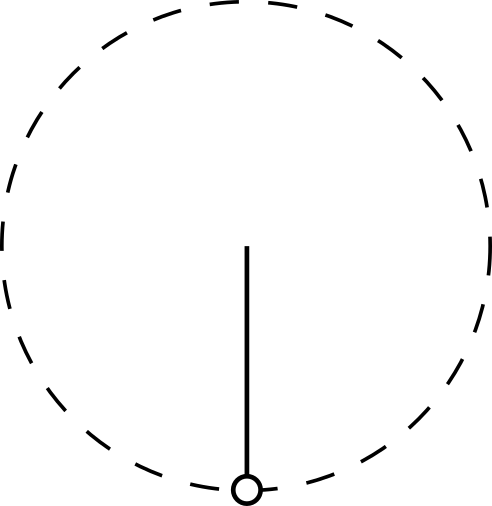
\includegraphics[width=.5\linewidth]{Images/mass_pendulum_eq1.png}
        \caption{Stable equilibrium}
        \label{fig:mass-pend-stable}
    \end{subfigure}%
    \begin{subfigure}{0.5\textwidth}
        \centering
        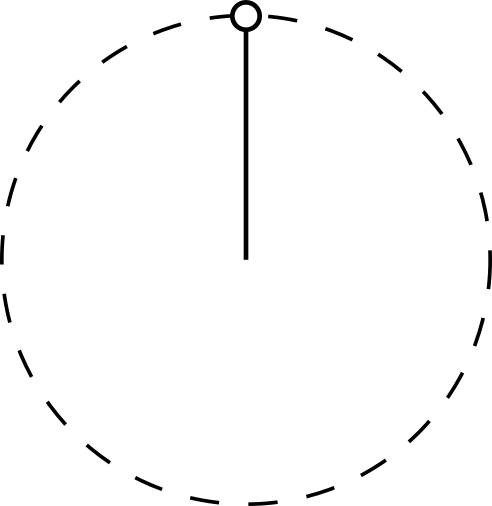
\includegraphics[width=.5\linewidth]{Images/mass_pendulum_eq2.png}
        \caption{Unstable equilibrium}
        \label{fig:mass-pend-unstable}
    \end{subfigure}
    \caption{Equilibria in mass pendulum setup}
\end{figure}

We get some rather interesting behaviour at $r = 0$, in the frictionless case. In this case we get a center which again should make sense. If there is no friction, then the pendulum continues swinging on its path ad infinitium. 